\documentclass[../thesis/thesis.tex]{subfiles}
\renewcommand{\baselinestretch}{1.5}\selectfont
\graphicspath{{../figs/ch4-vnaunc/}}

\begin{document}
	
\onlyinsubfile{\setcounter{chapter}{3}}

\begin{refsection}
\chapter[Evaluating Uncertainty in VNA Measurements]{Evaluating Uncertainty in Vector \\Network Analyser Measurements}

\section{Introduction}

The dramatic growth of radio-based devices and applications over the last 50 years has led to the VNA becoming a critical instrument in most laboratories. Many of these applications required both accurate and reliable measurements from these VNAs.  This is particularly so in areas such as manufacturing, calibration and testing.  This is often driven by requirements given in international Quality Management documents such as the ISO 9000 series of standards \cite{ISO9000} (for manufacturing and process control) and the ISO 17025 standard \cite{ISO17025} (for calibration and testing).

The requirements given in these international standards are for measurements that can be demonstrated as fit-for-purpose (in terms of the achievable level of accuracy, etc) and made traceable to the international system of units \cite{SI_2019, SI_2019B}.  These requirements were not trivial for a VNA due to the complicated nature of the VNA’s operating principles, for example the calibration mathematics. Combined with the available computing power and cost at that time, a full or rigorous evaluation of uncertainty for VNA measurements, per for example the ISO GUM document, was difficult and time-consuming. This led to much work by experts in this field to develop easier methods that addressed these needs in ways that were suitable for use by end-users in the manufacturing, calibration and testing communities.  Much of this work was undertaken by the ANAMET Technology Group (www.npl.co.uk/anamet) during the 1990s.  This resulted in a series of reports \cite{ANAMET_1996, ANAMET_1998, ANAMET_1999} describing the development of a guidance document that gave a procedure for assessing the performance of calibrated VNAs.  The resulting guidance document \cite{EA_2000} was published by the European co-operation for Accreditation (EA, www.european-accreditation.org) so that laboratories operating to the ISO 17025 standard and/or ISO 9000 series of standards could implement the method for their own purposes.  Ownership of this EA document was later transferred to the European Association of National Metrology Institutes (EURAMET) and re-published \cite{EURAMET_2011} as part of their Calibration Guides series of documents. This document, along with the recent updated version, is available as a free download from the EURAMET web-site: www.euramet.org.

In addition to the EURAMET guide, VNA manufacturers have also produced their own advice for users to estimate the combined standard uncertainty in their measurements \cite{Hiebel_2008} and provided software tools in some cases \cite{KeysightUncTool, AnritsuUncTool}. Often this advice is based on the same methods presented in the EURAMET guide.

In more recent years rigorous evaluations of VNA uncertainty have become possible, through both the efforts of NMIs and access to greater computing resources. The difference between the previous approaches (which we will call ``residual error'' evaluations) and rigorous evaluations concerns the way in which uncertainty contributed by the VNA calibration is estimated and included in the measurement model. The two methods will be discussed later in this Chapter. Figure \ref{ch4_fig_vna_model} illustrates the general structure of VNA uncertainty sources and evaluation, from which each component will now be explained.

\begin{figure}
	\centering
	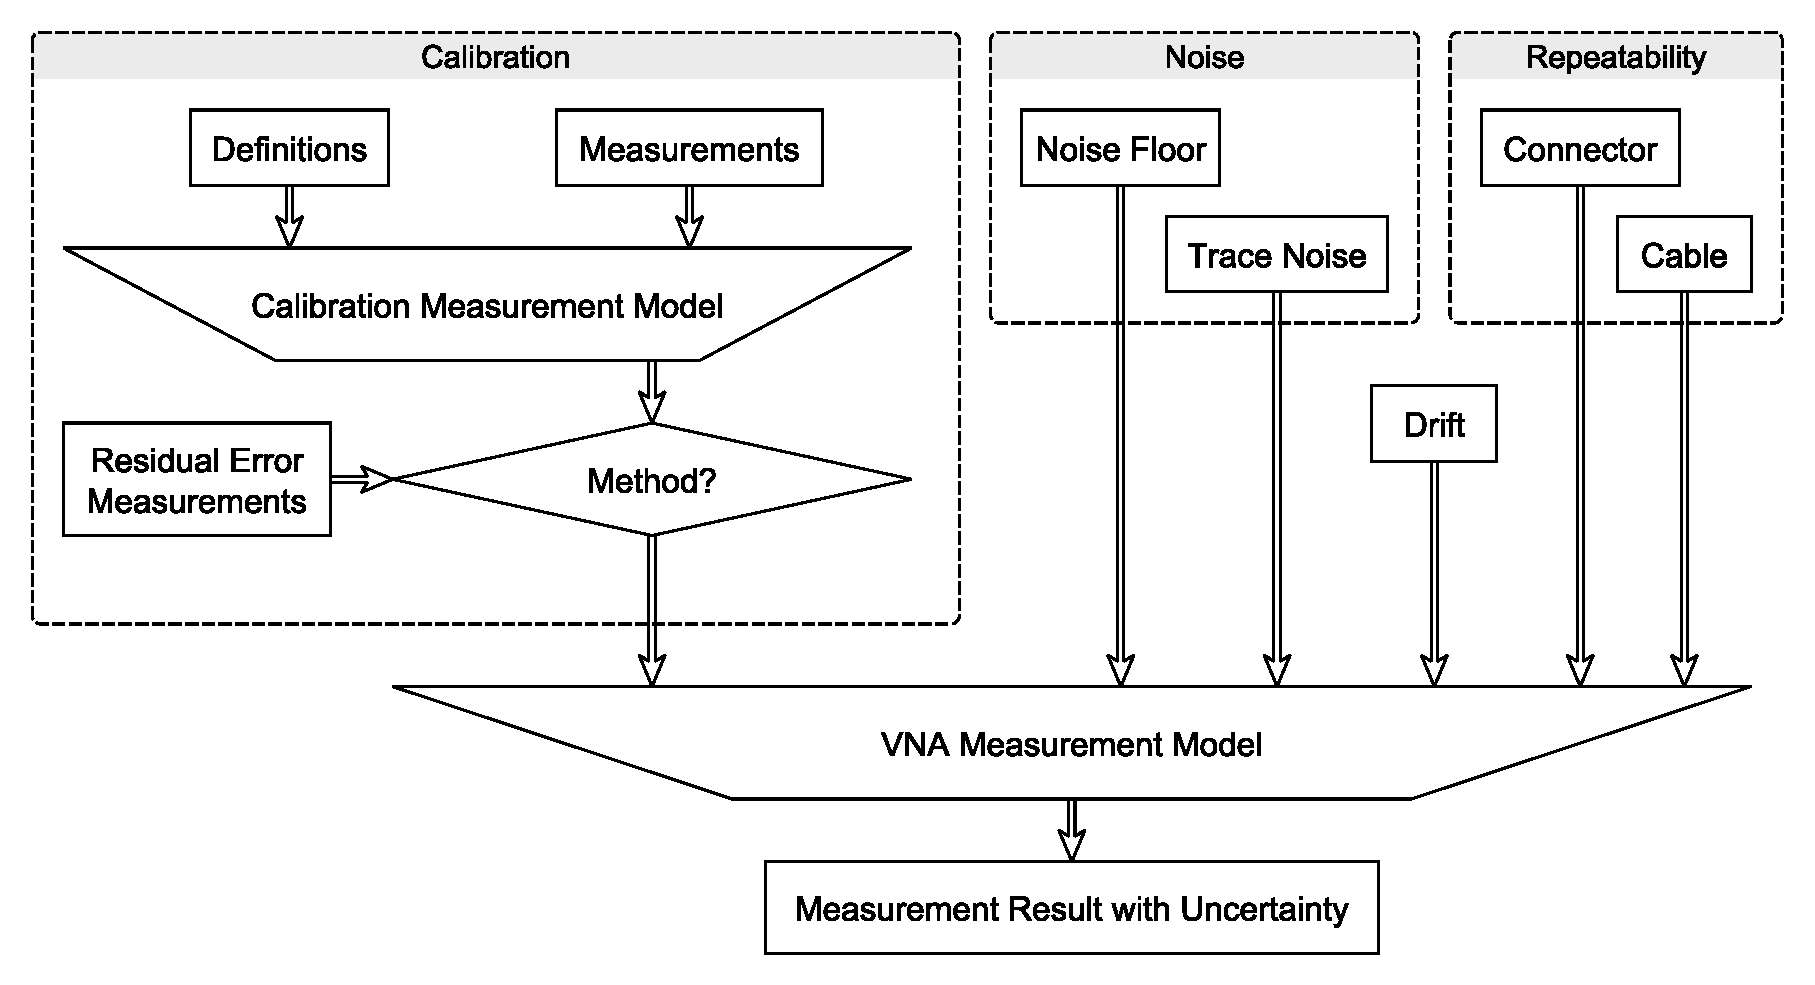
\includegraphics[width=\textwidth]{vna-model.pdf}
	\caption{Structure of VNA uncertainty evaluation. Input quantities are shown at the top of the diagram, grouped where applicable. Uncertainties from the calibration are either evaluated directly (rigorous/full evaluation) or are estimated after the calibration has been performed (``residual error'' evaluation). Typically the calibration measurement model is processed as part of the VNA measurement model, but it is shown separately here to distinguish the difference between VNA uncertainty evaluation methods.}
	\label{ch4_fig_vna_model}
\end{figure}

\section{VNA Measurement Model Input Quantities}
\subsection{Calibration Standards}

In order to perform the calibration, or error correction, of a VNA as described in Chapter 2, we must compare measurements of impedance standards to definitions of their true values in order to obtain error coefficients. It is interesting that although sources of error in the calibration cover both systematic and random types, when the calibration is performed and these quantities are measured, any random errors are captured in the evaluated combined uncertainty, which itself is purely systematic.

\subsubsection{Definitions}

Because the definitions of impedance standards are based on prior measurements, and all measurements include uncertainty, they are also included as a source of uncertainty in the VNA measurement model. We will now look at how uncertainty can be included in the three types of standard definition commonly used in VNA calibration routines.

\paragraph{Databased Definitions}

The simplest definition of an impedance standard is the databased definition. The standard is characterised by measurement on a VNA which has been calibrated to a suitable accuracy, i.e. using standards which are at an appropriate position in the traceability chain (closer to the primary standard). The combined standard uncertainty of the characterisation is then provided with the estimates as the definition of the standard.

It is important to characterise the standard across a suitable frequency range, usually the entire range for which it can be applied. In addition to the combined standard uncertainty, the covariances between the real and imaginary components of the measured s-parameters can also be included in the standard definition for more accurate uncertainty evaluations in measurements using the standard [RidlerSalterEtc]. If the standard will be used to calibrate VNAs producing results to be used in time-domain studies or multi-harmonic studies (i.e. nonlinear work), then ideally covariances between s-parameters for each frequency should be included. However, this is something which would consume a lot of data storage and the saving of this information is not supported by VNAs at this time.

\paragraph{Polynomial Model Definitions}

In order to reduce the information required to accompany the standard, one-port models are often defined as coefficients of a polynomial fit between reflection coefficient and frequency. This characterisation is performed by the manufacturer and the coefficients are available in the user manual or specification sheet for the impedance standards. Testing is performed by the manufacturer to ensure that the supplied standards do not deviate from this characterisation. Similar to the databased definition, care must be taken to ensure the characterised polynomial fit is valid across a suitable frequency range.

An example of a short-circuit polynomial fit, as defined in \cite{Keysight_2016}, is

\begin{align}
	L_\textrm{S} &= L_0 + L_1f + L_2f^2 + L_3f^3, \\
	Z_\textrm{S} &= j2\pi fL_\textrm{S}, \\
	\Gamma_\textrm{S} &= \frac{Z_\textrm{S} - Z_\textrm{r}}{Z_\textrm{S} + Z_\textrm{r}},
\end{align}

where $L_\textrm{S}$ and $Z_\textrm{S}$ are the respective inductance and impedance of the short-circuit, $L_n$ are coefficients provided by the definition of the standard,  $Z_\textrm{r}$ is the reference impedance and $\Gamma_\textrm{S}$ is the reflection coefficient of the short-circuit at frequency $f$. A similar model is used for open-circuits, with the inductive component replaced with a capacitive one.

Although no manufacturers are yet providing uncertainties with the polynomial coefficients supplied in their standard definitions, some have included the ability for future incorporation in the data file structure. In addition to uncertainty originating from the measurement of the standard, there will also be uncertainties relating to the error of the polynomial fit. Because of this, the polynomial definition is typically the least accurate type of standard definition, however it is popular due to the portability of the small number of coefficients which can be defined for the entire set of manufactured models.

\paragraph{Physical Definitions}

Typically understood as the most accurate, physically defined standards use robust geometric models to calculate their impedances from dimensional measurements. Models are available in coaxial transmission line for short-circuits, open-circuits and arbitrary line lengths. Good examples of these models and their derivations can be found in \cites{Keysight_2016}[Appendix C]{Lewandowski_2010}. Matched loads are more difficult to accurately model and so they are typically included as a databased standard, even if the other standards are physically defined. In order to avoid this issue, the TRL calibration can be used, which requires standards that can all be physically defined. This combination of calibration model and standard definition is commonly used by NMIs when performing traceable characterisations of other standards (i.e. databased definitions).

To obtain uncertainties in the reflection coefficients of physically defined standards, which are the measurands which we would then like to use as input quantities to the VNA uncertainty evaluation, an additional uncertainty evaluation must be performed. This takes the estimates and uncertainties of the dimensional measurements of the standards and propagates them through the measurement model (the geometric model relating dimension and frequency to reflection coefficient) to obtain the reflection coefficients with uncertainties required.

Dimensional measurements of the standards are usually supplied by the manufacturer for TRL calibration kits, but like the other definition types can be supplanted by recent measurements performed by NMIs or calibration providers. Another benefit of physically defined impedance standards is that their definition is valid over their entire valid frequency range, removing the risk associated with databased and polynomial definitions.

Covariance information is not required to be supplied by the definition because the dimensional measurements should be uncorrelated (they are separately manufactured parts). During the uncertainty evaluation to obtain the reflection coefficients of the standards, covariances between both the complex impedance components and those at different frequencies are calculated. Therefore physical definitions are well suited to both portability, accuracy and use with time-domain or nonlinear measurements.

\subsubsection{Measurements}

During the calibration procedure the impedance standards are measured. Although the VNA is not yet calibrated, it is still performing a measurement (with reference to an arbitrary impedance) and so all of the sources of uncertainty additional to those from the calibration will be included. Sources such as noise are therefore counted several times during a VNA measurement due to their inclusion in the prior calibration measurements. Because of this, it is important to include correlations where possible for these sources as they will have a greater impact on the combined standard uncertainty of the result.

\subsection{Noise}

Noise plays an important role in RF and microwave engineering. It is a random effect which occurs at a fundamental level and cannot be corrected for, both in communication systems and instrumentation. Wireless transmission systems lose a large amount of signal through propagation and receivers must be designed to handle signals with a considerable amount of noise. Likewise, VNA transmission measurements of devices with high isolation or reflection measurements of devices with low insertion loss also exhibit a low signal-to-noise ratio. To obtain accurate results, it is therefore important for VNA manufacturers to provide instruments with low noise sources and receivers. To ensure that measurements which are more susceptible to noise are accurate, it is also important to quantify the noise associated with the measurements so that it can be included as a contribution to their combined standard uncertainties.

The amount of electrical noise in VNA measurements is a sum of thermal noise and contributions from the VNA components. Thermal noise, caused by the random motion of free electrons in a conducting material by heat, is specified as $4\times 10^{21}$ W/Hz ($-174$ dBm) \cite{Hiebel_2008}. The intermediate frequency bandwidth (IFBW) setting on the VNA controls the frequency range of signals being measured at each discrete point in the sweep, and can typically be set from $1$ Hz to more than $10$ kHz. It is this figure which multiplies the thermal noise to provide a theoretical minimum noise floor if we assumed the VNA did not contribute any noise itself. The disadvantage of a very low IFBW is that the VNA takes longer to perform the measurement, so there is a compromise between speed and accuracy. This provides a good example of where uncertainty evaluation can have a direct perceivable benefit to measurement accuracy - if the IFBW is reduced the uncertainty due to noise should also reduce. By quantifying the uncertainty the engineer can make an informed decision as to what value to set the IFBW, which could have expensive time implications in a test environment.

In addition to the thermal noise, the VNA contributes to the noise level from the source, receiver and other test set components (i.e. local oscillator phase noise). Setting attenuators to lower values will improve noise as resistors add additional thermal noise to the measurement. The noise figure (NF) of a VNA is typically quoted in the specifications, and can be used with the thermal noise to calculate the theoretical noise level of the VNA measurement \cite{Hiebel_2008}:

\begin{equation}
	L_\textrm{N} = -174 \textrm{dBm} + NF + 10\log(S_\textrm{F})\textrm{dB} + 10\log\left(\frac{B_\textrm{IF}}{\textrm{Hz}}\right)\textrm{dB}
\end{equation}

For the purposes of uncertainty evaluation, VNA noise level is measured on the instrument itself and is typically included in the measurement model as two input quantities, noise floor and trace noise. It is important that the VNA settings (IFBW, test port power, averaging) are the same as will be used for the DUT measurements, and that no calibration is applied.

\subsubsection{Noise Floor}

The noise floor is a term used to describe the noise present in the measurement with no external signal present. It can be measured with a matched load connected directly to the test port and should not include any noise contribution from the VNA source. Alternatively it can be measured from the transmission measurements of a 2-port VNA while short-circuits or open-circuits are connected for the trace noise measurement described below. Many measurements are made (\cite{EURAMET_2011} suggests a few hundred) and the standard deviation is calculated for each frequency point.

\subsubsection{Trace Noise}

Trace noise includes noise contributions from the VNA source and is a function of the measured power at the receiver. It is measured with a short-circuit or open-circuit connected directly to the test port.

\subsection{Repeatability}

Both the DUT connections and movement of the VNA port extension cables contribute uncertainty to the repeatability of VNA measurements. These errors vary when a different device is connected to the test setup, and are included for both the DUT measurement and the measurements of the impedance standards during calibration.

\subsubsection{Connections}

Connector repeatability is a fundamental quality of precision RF and microwave connectors. It can have a significant impact on DUT measurements if the response of the connector varies between multiple connections, and this perturbs the reference impedance of the calibrated VNA away from $50$ Ohms if this occurs between connecting calibration standards.

In order to measure connector repeatability uncertainty, a short-circuit can be connected to a calibrated VNA and the reflection coefficient measured. Measurements are then repeated, reconnecting the short at a different azimuthal rotation each time. This should be done at least three times with rotations of $120\deg$, although some guidance recommends up to 16 times\cite{EURAMET_2011}.

\subsubsection{Cable Stability}

When test port cables are flexed, their physical dimensions are perturbed, which in turn affects their s-parameter response. Specialist VNA test port extension cables are provided to mitigate the effects of cable flexure, although they do not remove them. It is therefore advisable to restrict the movement of these cables using clamps and supports, and also to wait a suitable time (typically 30 seconds or more) for stresses in the internal dielectric to settle.

Cable stability can be characterised in different ways depending on the VNA measurement model used. The general method is to perform repeated measurements while moving the cable between a range of positions which cover the maximum extent the cable will move during measurements of the calibration standards and DUTs. Specifically, some methods connect a short-circuit to each test port cable, and others connect the cables together to perform the characterisation (if used for a two-port measurement).

\subsection{Drift}

Drift does not strictly fit into the random or systematic error category, because it can vary over the course of measurements but is not random in nature. The dominant cause of drift is environmental conditions, especially temperature variations. Temperature affects the physical dimensions and s-parameters of RF components in the test setup and also the behaviour of the electronic devices inside the source and receiver - both of which perturb the result of the measurement.

Drift is an important source of uncertainty to include for measurements occurring over a long period of time after calibration, especially those in a test environment or in standards labs while performing a large number of repeat measurements. In order to minimise the effects of drift, the room which the VNA is located in should have good temperature control and all the equipment should have been powered on for at least 24 hours for their internal temperatures to settle.

In order to measure uncertainty due to drift, many repeat measurements are performed over a long period (24 hours or more). This procedure can be automated so that an operator is not required for the entire period. An alternative method of including uncertainty due to drift can be achieved by performing calibration measurements of standards both before and after the DUT measurements. The calibrations can be averaged and a crude standard deviation obtained.

\subsubsection{VNA Linearity}

One source of VNA measurement uncertainty which is still included in some evaluations is that from the nonlinearity of the receivers. However, in modern VNAs automatic level control corrections are sufficiently accurate to allow this error to be neglected \cite{Rytting_2001, Martens_2007}.

\section{Simplified Residual Model for VNA Uncertainty Evaluation}
\subsection{Method}

The EURAMET Guide \cite{EURAMET_2011} presents a process for evaluating the uncertainty of measurements performed on a calibrated VNA, allowing users to verify that values measured using the instrument are of acceptable accuracy. This process involves measuring a selection of dominant contributions to measurement uncertainty and combining them appropriately. Contributions include both systematic errors, which remain constant over the period of measurements, and random errors, which do not.  The error model for voltage reflection coefficient ($\Gamma$) measurements performed with a VNA is represented in \cite{EURAMET_2011} by the following equations for one-port (1) and two-port (2) measurements:

\begin{align}
U_{\Gamma} &= D + T\Gamma + M\Gamma^2 + R_{\Gamma}\\
U_{\Gamma} &= D + T\Gamma + M\Gamma^2 + R_{\Gamma} + S_{21}^2\Gamma_L
\end{align}

where $U_{\Gamma}$ is the combined uncertainty in the measurement, $D$ is the residual directivity, $T$ represents the effect of tracking and nonlinearity, $M$ is the residual test port match (TPM), $\Gamma$ is the measured voltage reflection coefficient, $R_{\Gamma}$ is the sum of all the random contributions, $S_{21}$ is the nominal attenuation of the device-under-test (DUT), and $\Gamma_L$ is the residual load match. The most significant systematic error contributors to the measurement uncertainty are, in most cases, the directivity and TPM.

To measure $\Gamma$, the VNA must separate reflected and incident voltage waves and then sample them using complex receivers. However, various components in the signal path may cause a portion of the incident wave to leak into the reflected wave receiver without having reached the DUT. This directivity error should be removed by applying correction terms extracted during the VNA calibration. However, as no calibration will be perfect, some residual directivity error will remain (referred to as effective directivity in \cite{EURAMET_2011}). To measure the residual directivity, a matched load can be connected to the test port being assessed. This should theoretically reflect none of the incident wave and the only voltage present at the reflected wave receiver should be due to the residual directivity. In practise, the match of the load will never be perfect, so it is likely that using this method the residual directivity will typically be either over- or underestimated. An improved method, used in \cite{EURAMET_2011} and widely accepted for use with coaxial measurements, is called the ‘ripple extraction technique’. This uses a similar principle to measure the residual directivity, but significantly improves the accuracy of the residual error evaluation. An illustration of its method is provided in Figure \ref{ch4_fig_ripple1}.

\begin{figure}
	\centering
	\begin{subfigure}{\textwidth}
		\centering
		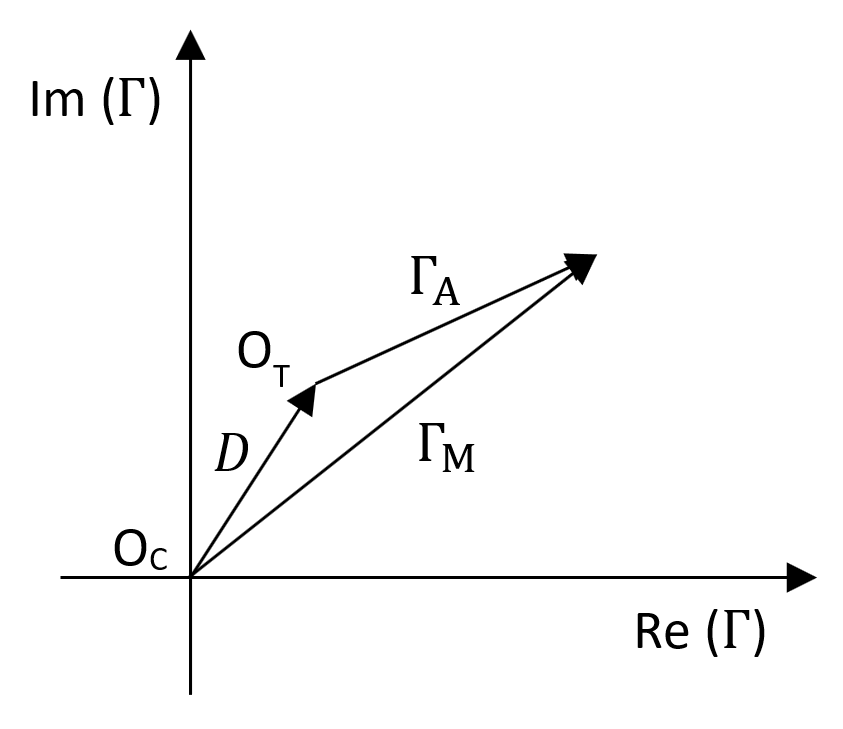
\includegraphics[width=0.32\textwidth]{Ripple1.png}
		\caption{When measured on the calibrated VNA, a perfect matched load would reveal the actual origin ($O_\textrm{A}$) on a polar plot of $\Gamma$ as offset from the calibrated origin ($O_\textrm{C}$) by the residual directivity ($D$). If a realistic matched load offset by a line section is instead measured, $\Gamma$ as measured by the VNA ($\Gamma_\textrm{M}$) will be the sum of the residual directivity $D$ and the actual $\Gamma$ ($\Gamma_\textrm{A}$). }
	\end{subfigure}
	\\
	\begin{subfigure}{\textwidth}
		\centering
		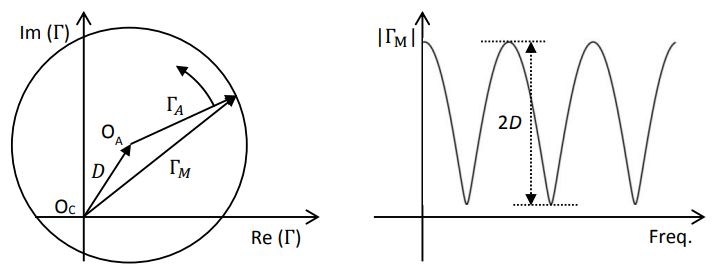
\includegraphics[width=0.75\textwidth]{Ripple2.png}
		\caption{As $\Gamma_\textrm{M}$ is measured across a swept frequency range, the phase change in the line increases causing the phase of $\Gamma_\textrm{A}$ to sweep also. This rotates $\Gamma_\textrm{A}$, resulting in ripples in the plot of $|\Gamma_\textrm{M}|$ against frequency. The magnitude of the ripples is equal to $2D$. }
	\end{subfigure}
	\\
	\begin{subfigure}{\textwidth}
		\centering
		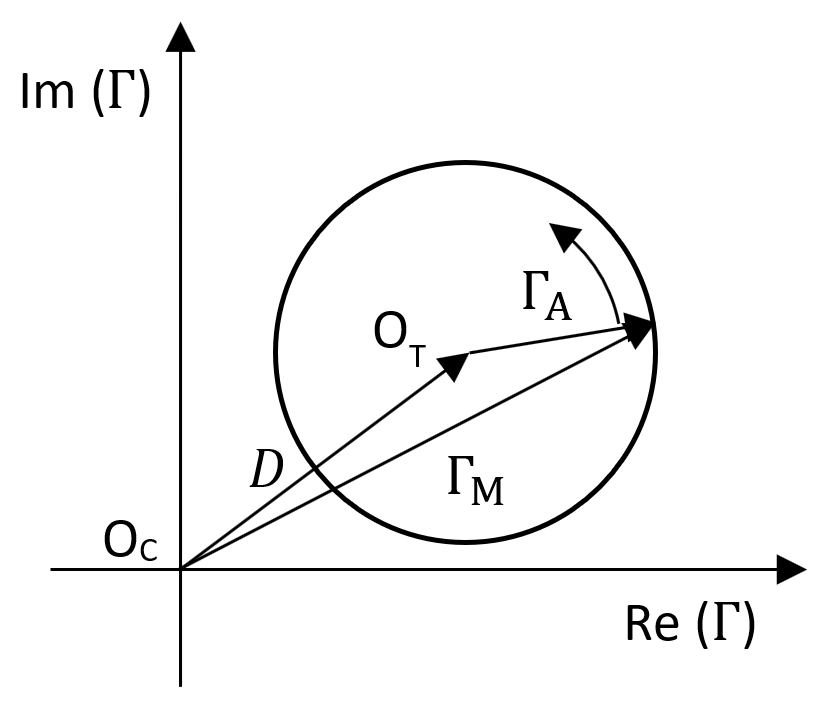
\includegraphics[width=0.75\textwidth]{Ripple3.png}
		\caption{However, if $\Gamma_\textrm{A} < D$, then the ripple magnitude is now $2\Gamma_\textrm{A}$ instead of $2D$ and the residual directivity as evaluated using the ripple extraction technique would be underestimated.}
	\end{subfigure}
	\caption{A graphical representation of the ripple extraction technique, including a possible failure mechanism.}
	\label{ch4_fig_ripple1}
\end{figure}

To perform the ripple extraction technique, a short length of line is connected to the test port, to the end of which is added a near-matched load covering the frequency range under test. The critical dimensions of the line section (length and radii) should be traceable to national standards and have a characteristic impedance
identical to that of the VNA setup. For these reasons a beadless airline is suggested in \cite{EURAMET_2011}. The load can be either the same as that used for calibration or another with $0.1 \ge |\Gamma| \ge 0.2$ (in linear units) to ensure that $|\Gamma| \ge |D|$. If $|\Gamma| < |D|$, then the measured residual directivity will be underestimated as explained by Figure \ref{ch4_fig_ripple1}. If the calibration matched load is used for the measurement, the small reflection from a second connection and any loss in the airline will cause $\Gamma$ to be greater than the residual directivity from the original measurement of the load. Alternatively, because $|\Gamma| < 0.1$ for the matched load used for calibration, using another load with a known higher $|\Gamma|$ ensures that there is no underestimate. Once the instrument has been configured, $\Gamma$ is measured and the magnitude plotted against frequency using a linear scale. A ripple will then be visible on the trace, from which the residual directivity can be calculated from:

\begin{equation}
D = \frac{\textrm{MRA}_\textrm{matched-load}}{2}
\end{equation}

For coaxial measurements as specified in \cite{EURAMET_2011}, there is a high probability that the condition required to avoid underestimation of $|D|$ is met. However, in order to assess the suitability of the technique in waveguide a method of assessing this condition has been used. By examining either a complex plot (polar or Smith chart) or a phase plot, the geometric symptom shown in Figure \ref{ch4_fig_ripple1} can be identified. When using a complex plot, the origin should lie within the circumference of the reflection coefficient trace for a valid determination of the residual error to be achieved. For any frequency range where it does not, the ripple technique provides an underestimation of the residual error. When using a phase plot, there will be regular wrapping of the reflection coefficient phase for frequency ranges where the residual error is correctly measured, whereas when underestimation occurs the phase will vary by $<180^\circ$ per period. An example of both plots are shown in Figure \ref{ch4_fig_dir}, where the result from the different load indicates an accurate residual directivity estimate across the entire measured spectrum, but the result from the calibration load shows an underestimate of the residual directivity is likely between 16 and 22 GHz. Either of these methods can be used to identify when a calibration and the ripple extraction technique needs to be repeated. If the repeat measurements still fail the test, then the choice of loads may need to be altered. 

\begin{figure}
	\centering
	\begin{subfigure}{0.45\textwidth}
		\centering
	    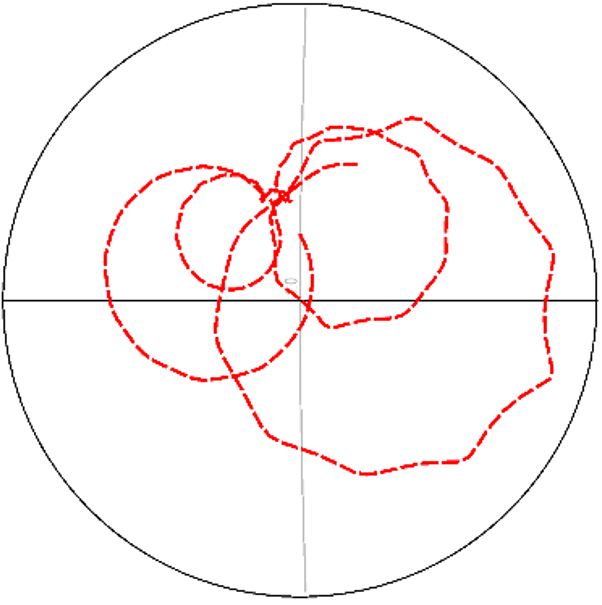
\includegraphics[width=0.9\linewidth]{dir-a.png}
	    \caption{A Smith chart representation, magnified about the origin, of the calibration load result.}
    \end{subfigure}\hfill%
	\begin{subfigure}{0.45\textwidth}
	    \centering
	    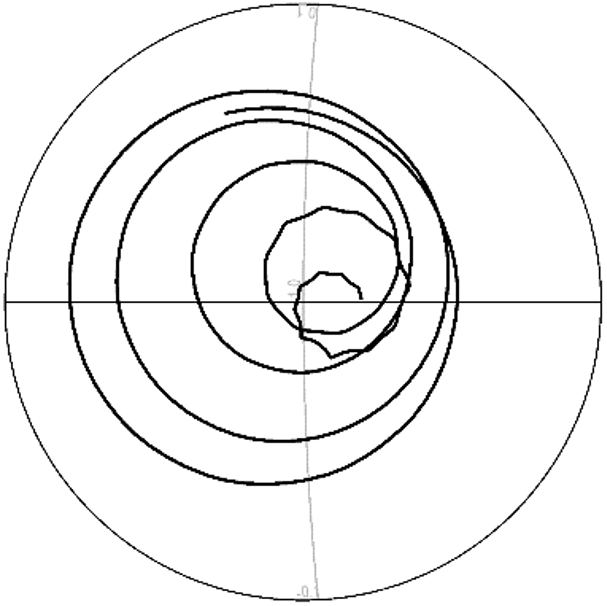
\includegraphics[width=0.9\linewidth]{dir-b.png}
	    \caption{Similar Smith chart representation of the different load result. The intersection of the two grid lines on the Smith charts represents the origin of the plot ($|\Gamma|=0$), and both are scaled separately for clarity.}
    \end{subfigure}
	\par\bigskip
	\begin{subfigure}{0.6\textwidth}
	    \centering
		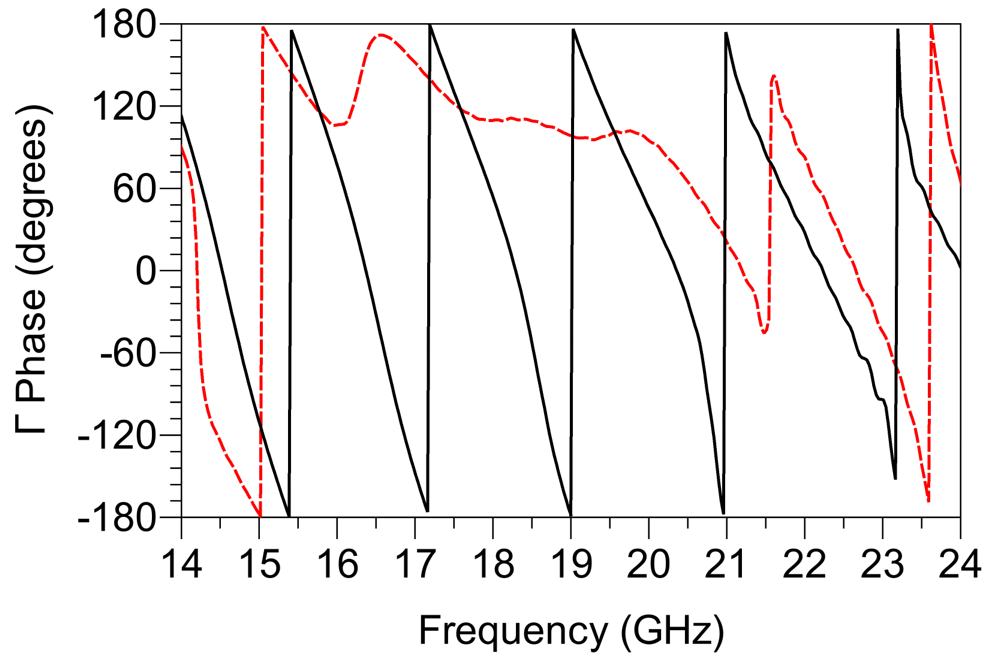
\includegraphics[width=\linewidth]{dir-c.png}
		\caption{Phase plot of both results, with the calibration load represented by the red dotted trace and the different load by the black solid trace.}
	\end{subfigure}
	\caption{Measurements of residual directivity plotted over the frequency range of 14--24 GHz performed in coaxial transmission line using both the load used for calibration and a load from a different calibration kit.}
	\label{ch4_fig_dir}
\end{figure}

TPM is caused by imperfections in the impedance match between components in the VNA setup. This causes delayed reflections that interfere with the DUT measurement and can provide false values. Calibration also corrects for TPM, but as with directivity some residual error will remain. To measure residual TPM, a short circuit is connected to the test port being assessed. This should reflect the entire incident signal and therefore maximise any reflections in the VNA setup. If residual TPM error is present then the measured $\Gamma$ will be $<1$. However, the short circuit may not provide a perfect reflection and so the ripple extraction technique is favoured for this measurement also.

To measure residual TPM using the ripple extraction technique, the same procedure as for residual directivity is followed but the matched load at the end of the line is replaced by a short circuit. A similar plot is acquired and the residual TPM is given by:

\begin{equation}
M = \frac{\textrm{MRA}_\textrm{short-circuit}}{2}
\end{equation}

Since the reflection coefficient for this measurement should be close to 1, there is no risk that this value will be greater than the true residual TPM and cause an underestimate as can be the case for residual directivity. This is shown in Figure \ref{ch4_fig_tpm}, where the origin of the Smith chart is clearly inside the circular trace (Figure \ref{ch4_fig_tpm}a) and the phase consistently wraps across the entire measured spectrum (Figure \ref{ch4_fig_tpm}b).

\begin{figure}
	\centering
	\begin{subfigure}{0.37\textwidth}
		\centering
		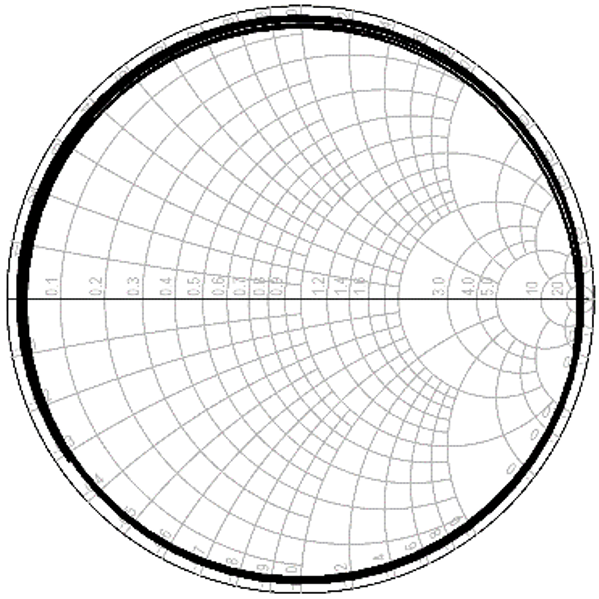
\includegraphics[width=0.9\linewidth]{tpm-a.png}
		\caption{Smith chart representation of the result when using the calibration short-circuit. The result when using a short-circuit from a different calibration kit appears almost identical.}
	\end{subfigure}\hfill%
	\begin{subfigure}{0.6\textwidth}
		\centering
		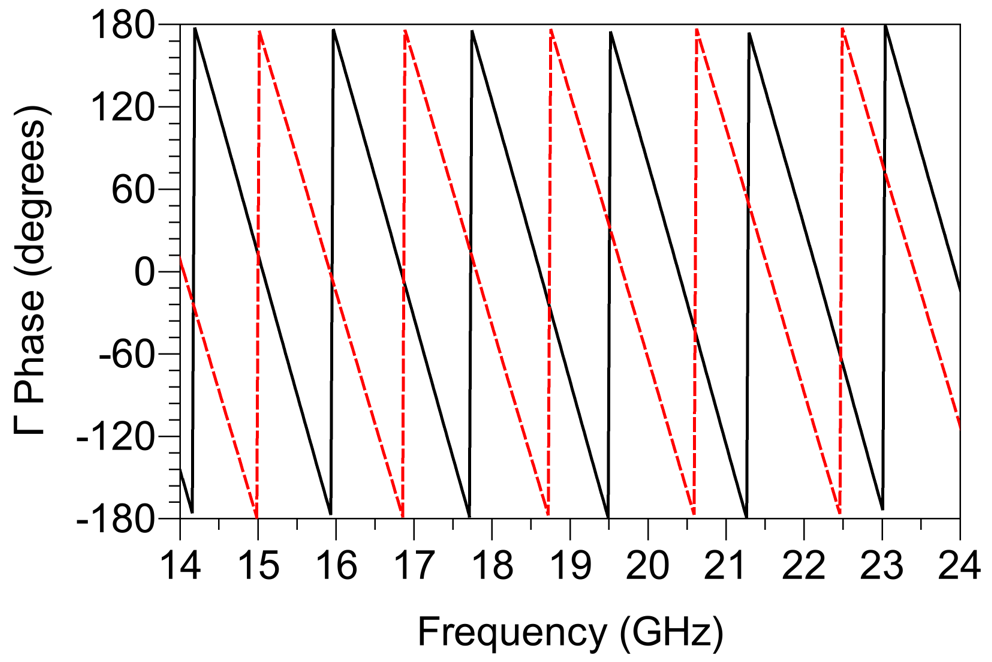
\includegraphics[width=0.9\linewidth]{tpm-b.png}
		\caption{Phase plot of the results when using the calibration short-circuit (dotted red trace) and the different short-circuit (solid black trace).}
	\end{subfigure}
	\caption{Measurements of residual TPM plotted over the frequency range of  14--24 GHz performed in coaxial transmission line.}
	\label{ch4_fig_tpm}
\end{figure}

To perform the technique for both described residual error sources requires just three components: A short circuit, matched load, and a short section of line. These components are realizable in both coaxial and rectangular waveguide, so the technique should be physically possible to perform in waveguide setups. The technique can be applied to any type of calibration – for example three-known-loads and thru-reflect-line (TRL). In coaxial, the short-open-load-thru (SOLT) variant of the former is used. However, in waveguide an open circuit is not straightforward to realise or widely adopted, so a common variant of SOLT calibration which uses an offset short (SOSLT) will be used instead.

\subsection{Application to Waveguide VNAs}

Although both the EURAMET guide and VNAs using rectangular metal waveguide test ports have both existed for many years, there was no published evidence that the methods employed in the guide (the ripple technique) could be successfully applied to those measurements. The author undertook an investigation into this during the degree where they compared residual error measurements in coaxial line to those in waveguides at frequencies ranging from 8.2 GHz to 750 GHz (submillimetre-wave). This section presents the results of the subsequent papers \cite{Stant_2016_Coll, Stant_2017}.

\subsubsection{Coaxial Transmission Line and Microwave Waveguide}

The ripple extraction technique was first performed on coaxial line in accordance with the EURAMET Guide \cite{EURAMET_2011} instruction as described in the previous section. The guide itself provides a range of typical values for both residual directivity and TPM ripple measurements with which our results can be compared to ensure that the process was followed correctly. All measurements presented in this investigation were acquired using a Keysight 5247A PNA-X instrument fitted with 1.85 mm ports attached to flexible port extender cables with rugged connectors. The coaxial measurement setup used a 75 mm beadless airline and the calibration kit matched load and short circuit. Figure \ref{ch4_fig_coax} shows the ripple trace obtained by plotting $|\Gamma|$ against frequency for residual directivity and TPM measurements using an SOLT calibration. Apart from the dominant ripple, other variations in $|\Gamma|$ are due to the imperfect response of the matched load and the beadless line. The results of the measurements, along with the expected ranges provided in \cite{EURAMET_2011}, are presented in Table \ref{ch4_table_coax}. It can be seen that the measured values for the coaxial line setup fall within the typical ranges specified by \cite{EURAMET_2011}.

\begin{figure}
	\centering
	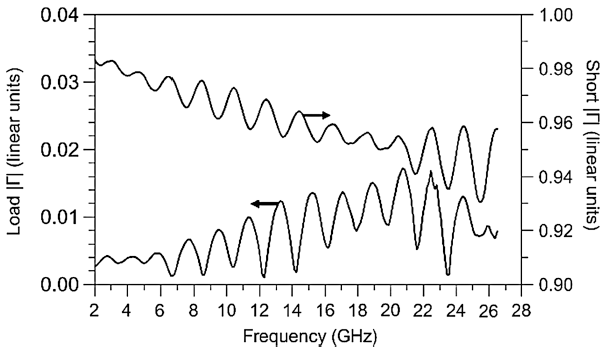
\includegraphics[width=0.65\textwidth]{coax.png}
	\caption{Magnitude of the reflection measurement of a matched load and a short-circuit offset by a length of coaxial line. The VNA was calibrated using the SOLT method.}
	\label{ch4_fig_coax}
\end{figure}

\begin{table}[]
	\begin{tabular}{lllll}
	\hline
	Cal. type       & \multicolumn{2}{l}{Residual directivity} & \multicolumn{2}{l}{Residual TPM} \\
	& Port 1              & Port 2             & Port 1          & Port 2         \\ \hline
	SOLT            & 0.008               & 0.009              & 0.014           & 0.010          \\
	TRL             & 0.008               & 0.007              & 0.002           & 0.002          \\
	EURAMET guide \cite{EURAMET_2011} & 0.002--0.02         & 0.002--0.02        & 0.005--0.02     & 0.005--0.02    \\ \hline
\end{tabular}
	\caption{Residual directivity and TPM values obtained for 3.5 mm coaxial line VNA calibrations as measured by the ripple extraction method. Both SOLT and TRL calibration techniques were assessed. The range of representative residual error values from \cite{EURAMET_2011} has also been included for comparison.}
	\label{ch4_table_coax}
\end{table}

 The same method was applied to two types of centimetre band waveguide, WR-90 and WR-42. These waveguides have usable frequency ranges of 8.2--12.4 GHz and 18.0--26.5 GHz respectively. To avoid the effects of non-propagating (evanescent) modes created by the waveguide to coaxial adapter, an appropriate length of straight waveguide was attached to each adapter where possible and the measurement planes defined at the end of the lines. The results of the ripple extraction technique for the two waveguide sizes are shown in Table \ref{ch4_table_WG16}:

\begin{table}[]
	\begin{tabular}{lllllll}
		\hline
		Frequency, GHz & Waveguide size & Cal. type & \multicolumn{2}{l}{Residual Directivity} & \multicolumn{2}{l}{Residual TPM} \\
		&                &           & Port 1              & Port 2             & Port 1          & Port 2         \\ \hline
		8.2--12.4      & WR-90           & SOSLT     & 0.005              & 0.004             & 0.007          & 0.006         \\
		&              & TRL       & 0.003              & 0.006             & 0.002          & 0.002         \\
		18--26.5       & WR-42           & SOSLT     & 0.003              & 0.004             & 0.010          & 0.005         \\
		&              & TRL       & 0.002              & 0.002             & 0.002          & 0.001         \\ \hline 
	\end{tabular}
	\caption{Residual directivity and TPM values of WR-15 and WR-05 waveguide VNA calibrations as measured by the ripple extraction method. Both SOSLT and TRL techniques were used to calibrate the VNA.}
	\label{ch4_table_WG16}
\end{table}

\subsubsection{Millimetre-wave Waveguides}

To perform measurements at frequencies above 50 GHz, a range of external frequency extender heads were attached to the VNA. These extender heads included a line section attached to each test port of suitable length to avoid effects caused by evanescent modes that may exist close to the test port. To study the performance of the ripple extraction technique at millimetre wavelengths, WR-15 and WR-05 waveguides were chosen. These waveguides have operating frequency ranges of 50--75 GHz and 140--220 GHz respectively. The results of the ripple extraction are shown in Table \ref{ch4_table_WG25}:

\begin{table}[]
	\begin{tabular}{lllllll}
		\hline
		Frequency, GHz & Waveguide size & Cal. type & \multicolumn{2}{l}{Residual directivity} & \multicolumn{2}{l}{Residual TPM} \\
		&                &           & Port 1              & Port 2             & Port 1          & Port 2         \\ \hline 
		50--75         & WR-15          & SOSLT     & 0.002               & 0.002              & 0.018           & 0.017          \\
		&                & TRL       & 0.002               & 0.002              & 0.009           & 0.007          \\
		140--220       & WR-05          & SOSLT     & 0.008               & 0.009              & 0.019           & 0.024          \\
		&                & TRL       & 0.007               & 0.008              & 0.021           & 0.015          \\ \hline
	\end{tabular}
	\caption{Residual directivity and TPM values of WG25 and WG30 waveguide VNA calibrations as measured by the ripple extraction method. Both SOSLT and TRL calibration techniques were measured.}
	\label{ch4_table_WG25}
\end{table}

\subsubsection{Submillimetre-wave Waveguides}

The final stage of the investigation studied the ripple extraction technique when applied to submillimetre wavelength VNA setups. The waveguide chosen for these measurements was in the 500--750 GHz band (WR-1.5) for which only one frequency extender head was available. Owing to the requirement for a
through standard when using the TRL calibration method, only a three-known-loads calibration was performed, which was the one-port version of SOSLT (SOSL). The line section used was $\sim$25.4 mm in length and was part of a calibration and verification kit manufactured by Virginia Diodes, Inc. All waveguide flanges, apart from the short-circuit, used precision alignment dowels located above and below the aperture. Figure \ref{ch4_fig_setup} shows the setup used during the measurement of residual directivity, with a line and match connected to the frequency extender head. 

It can be seen that the residual directivity is significantly smaller than the residual TPM. By
assessing the phase wrapping of the ripple trace obtained for evaluating residual directivity, as shown in Figure \ref{ch4_fig_wm380}, the ripple extraction technique appears to be subject to the failure mechanism described in the previous Section 4.3.1 and illustrated in Figure \ref{ch4_fig_ripple1}c. The lack of phase wrapping across the entire operating bandwidth shows that the ripple extraction technique was not operating within the required assumptions necessary for the technique to be valid, and therefore provided an underestimate of the residual directivity. The calibration kit used for this experiment included two full sets of standards, so the matched load was swapped and the ripple extraction technique was repeated. The issue was not resolved by this change, so the calibration was repeated, this time using the other matched load. The ripple extraction technique was then performed with the matched load used for the original calibration. However, no combination of these components provided a valid residual directivity value as assessed by the phase wrapping method. A likely cause of this effect is the poor connection repeatability inherent in this waveguide size, using typical precision UG-387 flanges. If the waveguide apertures have a greater misalignment during calibration than when the ripple extraction technique is performed, the effect of the discontinuities can cause the calibration matched load to appear to have a higher $|\Gamma|$ than the one used for the ripple extraction technique (even if the opposite were in fact true). These conditions cause the residual directivity to be underestimated as explained in Section 4.3.1.

\begin{figure}
	\centering
	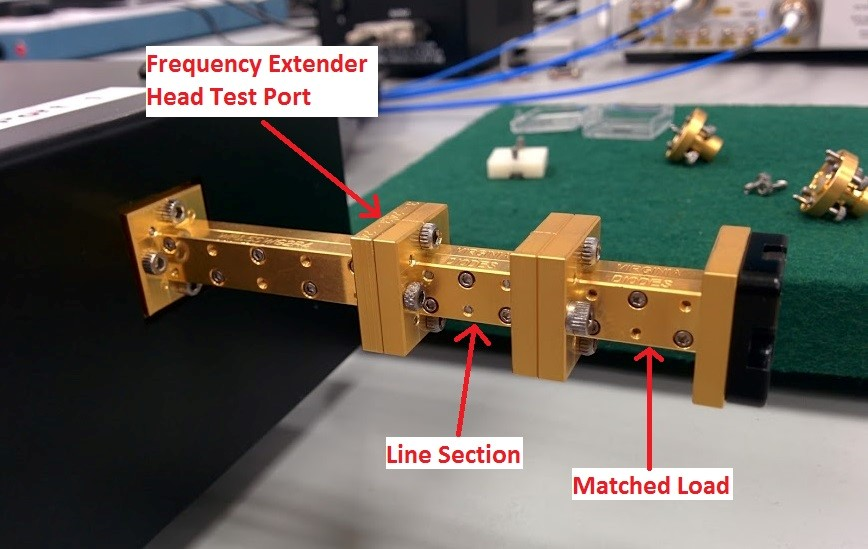
\includegraphics[width=0.65\textwidth]{setup.jpg}
	\caption{Test port setup used for residual directivity measurements in WR-1.5 waveguide.}
	\label{ch4_fig_setup}
\end{figure}

\begin{table}[]
	\begin{tabular}{lllll}
		\hline
		Frequency, GHz & Waveguide size & Cal. type    & Residual directivity & Residual TPM \\ \hline 
		500--750       & WR-1.5         & SOSLT Cal. 1 & 0.021                & 0.142        \\
		&                & SOSLT Cal. 2 & 0.025                & 0.065        \\ \hline 
	\end{tabular}
	\caption{Residual directivity and TPM values of two WR-1.5 waveguide VNA calibrations as measured by the ripple extraction method. Two similar types of calibration were performed using different standards from the same kit.}
	\label{ch4_table_WR1.5}
\end{table}

\begin{figure}
	\centering
	\includegraphics[width=0.65\textwidth]{wm380.png}
	\caption{Phase plot for a residual directivity evaluation performed in WR-1.5 waveguide using an SOSLT calibration.}
	\label{ch4_fig_wm380}
\end{figure}

\subsubsection{Waveguide Discontinuities}

When a discontinuity is present between two sections of rectangular waveguide, an increased reflection will be seen at the location of the join. There are three types of discontinuity possible in rectangular waveguide: E-plane and H-plane lateral displacements, angular displacement, and corner rounding. A report produced by Bannister \emph{et al.} \cite{Bannister_1989} presented the effects of these discontinuities at centimetre and millimetre wavelengths. Subsequent work by Kerr extended this using simulations \cite{Kerr_1999, Kerr_2010}. 

The error in $\Gamma$ contributed to by the effect of such discontinuities is proportional to wavelength, and therefore also the aperture size of the waveguide. At submillimetre wavelengths, the error has been shown to be considerable \cite{Williams_2011, Li_2012}. Recently, efforts have been made to improve the connection repeatability for waveguide at these wavelengths, and a new IEEE draft standard \cite{IEEE1785} presents three new connector types which significantly improves the alignment. Another potential improvement attempts to reduce misalignment errors during calibration by replacing the waveguide offset short with a radiating open, and new calibration algorithms have been developed to accompany this \cite{Arsenovic_2014}. The open standard must be very well characterised, and the technique has not yet seen widespread uptake.

\subsubsection{Discussion}

In centimetre-wave waveguides (WR-90, WR-42), the ripple extraction technique provided values of residual directivity and TPM similar to those obtained in coaxial line. This is not surprising as providing a good quality match is used for calibration and the connections are well made and aligned, both errors should not have significant contributions outside of the VNA itself. When extended to millimetre-wave waveguide, the residual errors were found to be larger, but still within the recommended values for coaxial lines. At submillimetre wavelengths, the two calibrations that were performed resulted in significant differences in the residual errors. A likely cause for these differences is the effect of discontinuities in the waveguide components (due to poor connection repeatability and demanding mechanical tolerances) used during the calibration, especially the matched load and offset short. Additionally, by studying the phase of the measured $\Gamma$, it was shown that the ripple extraction technique was not operating within required assumptions necessary for the technique to be valid and was therefore underestimating the true value of the residual directivity. The cause of this may also be related to the poor repeatability of the waveguide connection, causing the $\Gamma$ of the matched load used for the ripple extraction to be lower than that used for the calibration. Some effort were made to resolve this issue, but were unsuccessful. New improvements to submillimetre-wave waveguide flanges could significantly reduce this problem and allow the ripple technique to work more consistently with these very small waveguides.

A useful assessment method to test the validity of the ripple extraction technique was presented earlier in this paper, and should be performed whenever the technique is used. This assessment method views $\Gamma$ measured during the ripple extraction technique on either a phase plot, a polar plot or a Smith chart. When using a phase plot, this assessment has passed if the phase is seen to be wrapping across the operating bandwidth. When using a polar plot or Smith chart, this assessment has passed if the origin of the chart lies within the circumference of the trace. If the technique is deemed to have failed based on this assessment, the VNA should be recalibrated and the ripple extraction technique should be repeated. If this does not affect the assessment result, then the near-matched load or short-circuit used during the technique should be swapped with another (preferably known to have a higher $\Gamma$) and the ripple extraction technique repeated again. Only when this assessment has passed can the results from the ripple extraction technique be considered reliable.

\subsubsection{Conclusion}

This paper investigated the effectiveness of the ripple extraction technique when applied to rectangular waveguide measurements at centimetre, millimetre and submillimetre wavelengths. Typical values of residual directivity and TPM in these three ranges have been provided. For centimetre- and millimetre-wave waveguides the ripple extraction technique works as expected. Since the standards used in this investigation are commercially available and the calibration techniques are available on nearly all VNAs, the values of residual error given in this paper are considered representative and suitable for use as reference values by other users of similar types of measurement system, to compare their own values against. This is because the performance of these systems is usually dominated by the quality of the standards and the type of calibration technique that is used. However, this paper has also shown that the ripple extraction technique may not currently be a reliable way of measuring residual error in submillimetre wavelength systems. The effect of discontinuities at submillimetre-wave waveguide interconnections has been considered as a cause of this issue.

\section{Rigorous Models for VNA Uncertainty Evaluation}
\subsection{Method}

A rigorous evaluation of VNA uncertainty can be applied by using a measurement model which includes explicit relationships of the measurands to all input quantities. This is opposed to the residual model where the combined uncertainty from a collection of input quantities (relating to the calibration) is approximated. By including explicit relationships for all input quantities, the uncertainty evaluation can be directly traceable to primary standards.

There are several formulations of rigorous VNA measurement models in use, and most of them have been written into a software framework due to their complexity. The differences between the models are due to optimising the same mathematical relationships for different methods of processing. This section will now describe three popular VNA uncertainty frameworks.

\subsection{Keysight PNA-X Dynamic S-Parameter Uncertainty}

The Keysight PNA-X Dynamic S-Parameter Uncertainty option is an extension to the software provided on Keysight PNA-X VNAs. This software extension uses a separate graphical window to allow the user to manage sources of uncertainty (input quantities), which are then referenced by the VNA software to evaluate the combined standard uncertainty in the s-parameter measurements it produces.

Uncertainties for input quantities are provided in the form of calibration kits, cables and test ports. Mechanical standards in calibration kits can be characterised with uncertainty information by either measuring them on another PNA-X with the uncertainty software option, or supplied with that information from the manufacturer if they are Keysight products. Likewise, electronic calibration units from Keysight also include uncertainty characterisations in their definition files and can be loaded directly into the PNA-X software. Cable stability can be measured in a guided process through the uncertainty software and assigned to that cable identity for future use. Likewise, the test-port is used as an identity to store measurements of noise floor and trace noise, which are again measured through a guided process.

A calibration using uncertainty information is then performed, after which the VNA will perform measurements as normal. However, with the calibration applied it is possible to also view uncertainty information in real-time (i.e. calculated after every sweep) on the display. This can be in the form of error bars and lines showing standard deviations for scalar measurands like magnitude and phase, and also uncertainty ellipses showing standard deviations of complex values on polar plots or Smith charts.

The measurement model used within the PNA-X Dynamic Uncertainty Option is not fully disclosed, but it is based on a multi-port formulation developed by Garelli and Ferrero \cite{Garelli_2012}. This model rearranges the traditional calibration mathematics and creates new parameters which are very efficient for solving $n$-port calibration problems. This is a desirable property for commercial applications of VNAs where some communications products may require more than 24 ports to fully characterise their s-parameters.

Uncertainty information is stored in several file formats. The ``.u$n$p'' format, similar to the ``.s$n$p'' format, contains s-parameter data for an $n$-port device along with uncertainties in their respective scalar components (either real/imaginary or magnitude/phase). The Databased Standard Definition ``.dsd'' format contains characterisations of calibration standards, which in addition to uncertainty data from the ``.u$n$p'' format includes information about the type of calibration standard which is used by the software to ensure calibrations are performed correctly. Finally, the ``.sdatcv'' file format can also be read from and written to, which is native to the VNA Tools II software explained shortly. 

A more detailed overview of the methods used in the software can be found in the product Application Note \cite{Keysight_2019}.

\subsection{METAS VNA Tools II}

VNA Tools II is a piece of standalone software developed by the Swiss NMI, the Federal Institute of Metrology (METAS) \cite{VNATools}. Based on an uncertainty propagation library called UncLib \cite{UncLib}, also by METAS, the software is not attached to a particular VNA but can instead drive instruments from several popular manufacturers, or post-process existing measurements.

The underlying uncertainty propagation library, UncLib, specialises in linear propagation of uncertainty according the method described in the GUM document introduced in Chapter 3. Monte Carlo propagation is also included in the library, but is not as well supported. VNA Tools II defines a rigorous VNA measurement model using mathematics functions from UncLib, to which it provides measurement data and processes the uncertainty evaluation \cite{Wollensack_2012}.

In addition to the uncertainty evaluation, VNA Tools II allows users to store collections of characterised cables and calibration standards, as well as record all measurements in a journal for both short-term reference and archiving evidence of traceability.

To store uncertainty information for s-parameter measurements, a new file format was invented for VNA Tools II, which uses the ``.sdatcv'' filename extension. This file format stores s-parameter data with covariances between the real and imaginary components for each parameter at a particular frequency. Covariance data of parameters between frequency points is not saved as this can create very large files for typical VNA frequency sweeps, and is not useful when evaluating measurement uncertainty in the frequency domain for devices operating linearly. As mentioned earlier, this file format is also supported by the Keysight PNA-X Dynamic S-Parameter Uncertainty option, allowing standards to be used between the two different software frameworks.

\subsection{NIST Microwave Uncertainty Framework}

The Microwave Uncertainty Framework (MUF) published by the US National Institute of Standards and Technology (NIST) is another software framework for evaluating uncertainty from an NMI \cite{MUFWebsite, Ginley_2016, Ginley_2017}. Similar to VNA Tools II, the software does not need to be used with a specific brand of VNA because it can read existing measurement files (e.g. s-parameters) and perform calibrations during post-processing. The facility is available, however, to control Keysight VNA instruments remotely which can automate long measurement tasks for metrology studies.

Because the MUF was written to support general RF and microwave metrology research at NIST, many measurement models are included in the framework, of which VNA measurement models are just a few. The framework is provided as a collection of individual applications: \textbf{Post-Processor} contains a library of measurement models which can be evaluated using either Monte Carlo or finite difference (including sensitivity analysis) propagation techniques. \textbf{Model} allows two-port components to be defined, which can be cascaded together using \textbf{Cascade} and have their numerical parameters (e.g. length, resistance) assigned with statistical distributions using \textbf{Parameter}. One-port devices such as impedance standards are modelled as two one-port devices back-to-back. \textbf{Combine} takes a series of repeated measurements as an input and produces an estimate with associated uncertainty, according to classical probability methods. Finally, the \textbf{VNA Uncertainty Calculator} is a customised version of \textbf{Post-Processor} which includes a graphical layout to simplify loading of the many input quantities required for the VNA measurement models. Separate models are included for VNAs with up to eight ports, and six calibration types are available \cite{Jargon_2019}.

The MUF does not propagate uncertainty using covariance information stored in conventional matrices. Instead, at first chance it converts uncertainty information into a set of Monte Carlo samples. The order of these samples is carefully preserved throughout subsequent calculations, which has the effect of propagating covariance information throughout the uncertainty evaluation. For example, when a physically-defined impedance standard is modelled with parameters assigned statistical distributions, the MUF will sample from each distribution, evaluate the model and produce a sample to be used as an observation of an input quantity. This sample-based preservation of covariance information is very useful for input quantities with strong correlations - for example the real and imaginary components of a complex s-parameter measurement. Rather than statistically averaging a set of repeat measurements to assign a single covariance value, as outlined in the GUM document, the repeat measurements are preserved so that the distribution of covariance information is also used during the uncertainty evaluation. For most types of uncertainty source in the MUF this benefit is not realised because Monte Carlo samples are synthesised from statistical definitions (e.g. models, parameters), but for large numbers of repeat samples the functionality is available. The side-effect of this benefit is that keeping all of the measurement data, or synthesised Monte Carlo samples, can consume a lot of memory. However, modern computing resources mean that the space requirement is no longer a difficulty.

One of the most flexible features of the MUF is that any user can define their own models and post-processors (both are measurement models). This allows the MUF to provide uncertainty evaluations for new methods of electromagnetic wave metrology and communication systems research \cite{Dortmans_2019, Gu_2019}.

\section{NVNA Uncertainty Evaluation}

It was explained in Chapter 2 that in order to measure nonlinear devices using a VNA, the absolute power and phase of the waves at all test ports must be known. For a VNA to obtain this information, it must undergo additional calibration steps involving a phase reference and power meter. In addition, for mixer-based VNAs (the type used throughout this work), a stable phase reference must be connected to another port of the VNA and measured alongside any DUT measurements. Each of these additional requirements add input quantities to the NVNA measurement model when compared to that of the VNA, and these will now be discussed.

\subsection{Phase Reference}

The phase reference used during calibration contributes both systematic and random error sources. Because it is used as a calibration standard, systematic error due to inaccuracies of the characterisation is a primary concern. This is especially true for the phase calibration where the coefficients calculated from the measurements of the reference it's characterisation have a linear relationship with the calibrated DUT waves. This is different to the relative calibration of the VNA, where at least some of the coefficients are the result of information from several different impedance standards, therefore reducing the impact of a single inaccuracy in the characterisation or measurement of a single standard. In addition, for measurements of nonlinear microwave (and millimetre-wave) devices, harmonics of interest can be well above 10 GHz, where the wavelength in a transmission line is short and connector and cable repeatability errors (i.e. random errors) can have a large effect on the accuracy of the phase calibration.

The second phase reference used during measurements with a mixer-based NVNA recovers the true phases of measured waves after the local oscillator frequency changes. This phase reference does not contribute systematic error because the absolute phase values are mathematically cancelled during calibration (when measuring the first phase reference) and therefore they do not need to be known. Random errors due to connector and cable repeatability are also insignificant when measuring this device because their contributions are also cancelled during calibration and the device is never reconnected or moved afterwards. Instead, for this phase reference the dominant uncertainty contribution is drift, because to quantify the varying local oscillator phase and correct the DUT measurements, the reference phase must be constant. For this reason commercially available phase references will typically use temperature-controlled electronics to minimise the drift of the produced harmonic tones, which improves the issue \cite{Jargon_2003}. Because this phase reference is driven by another source (usually from within the NVNA, e.g. a 10 MHz reference clock), the phase noise and amplitude of this source will also have a significant effect on the uncertainty contribution. Blockley \emph{et al.} provide an excellent review of this source of uncertainty and it's impact on NVNA measurements \cite{Blockley_2007}. The key finding of this review is that for measurements using an IFBW of 100 Hz or below, the uncertainty contribution of random errors originating from the phase reference is negligible for typical DUT measurements. Although for VNA measurements IFBW settings above 100 Hz can be common for wideband frequency sweeps, the harmonic nature of NVNA measurements means that the IFBW is typically 30 Hz or below, which satisfies the recommendation from \cite{Blockley_2007}

To provide a suitably accurate characterisation of the phase reference a sampling oscilloscope can be used to measure the output of the device \cite{Reader_2008}. This oscilloscope can be calibrated using electro-optic techniques traceable to primary standards \cite{Williams_2006, Hale_2009}. This service is provided by NIST for Keysight phase references and includes information on the uncertainty in the amplitude and phase of each measured harmonic \cite{Keysight_2017}. The covariances between these quantities are not included, however, which can significantly affect the combined uncertainty of some nonlinear DUT measurements, including those involving cross-frequency terms such as behavioural models described later in Chapter 5.

Therefore, for this project two phase references were taken to NIST and re-characterised. The results of this characterisation included covariance information between the tone measurements at different harmonics and therefore can be used in a rigorous evaluation of uncertainty for nonlinear behavioural models. Results of the characterisation are shown in Figures \ref{ch4_fig_comb} and \ref{ch4_fig_combunc}. Due to the considerable effort required to perform a characterisation using an electro-optically calibrated sampling oscilloscope, a new technique was trialled to characterise our phase references using an NVNA. The instrument was calibrated using a phase reference which already had a traceable characterisation including covariance information, from which the our phase references were then measured. This will produce a characterisation with larger uncertainties because an additional measurement has been included in the traceability chain. The results show uncertainties of around 0.5 degrees across the spectrum, with a considerable ripple in measured phase occurring above 35 GHz. The origin of this ripple was not found during the course of the project but occurred during de-embedding steps.

\begin{figure}
	\centering
	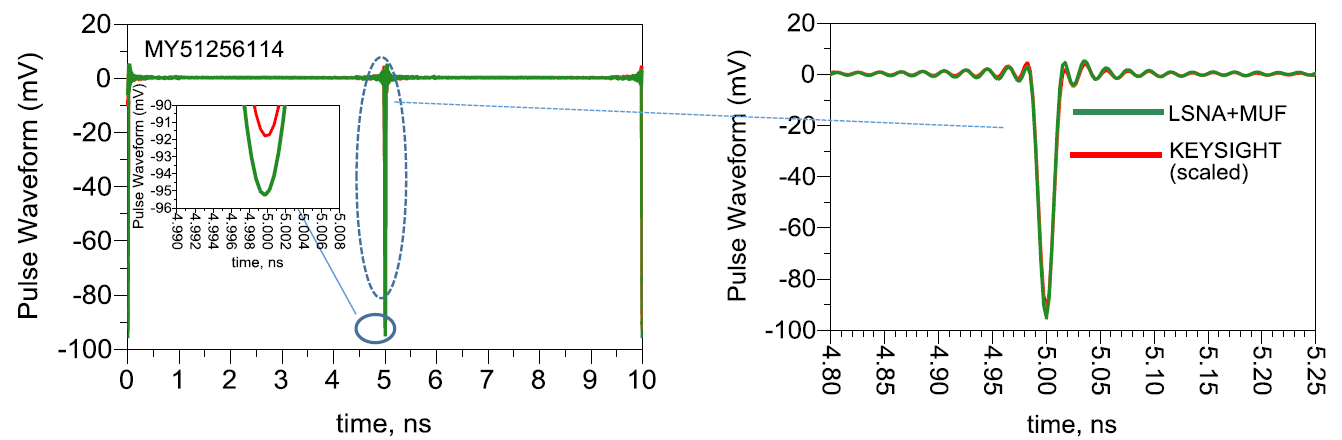
\includegraphics[width=\textwidth]{comb.png}
	\caption{Time domain representation of the pulse train which creates the harmonic comb in the frequency domain. The pulses repeat every 5 ns when the generator is driven with a 10 MHz stimulus. This figure is used with permission from a report produced by Gustavo Avolio, who performed the measurements at NIST. The results show good agreement between the Keysight characterisation stored on the device memory.}
	\label{ch4_fig_comb}
\end{figure}

\begin{figure}
	\centering
	\begin{subfigure}{\textwidth}
		\centering
		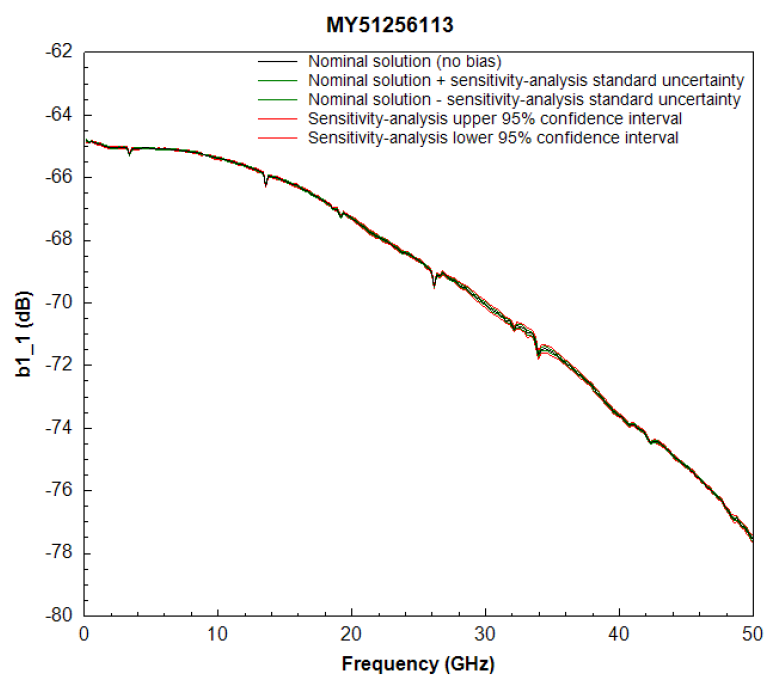
\includegraphics[width=0.62\textwidth]{combuncA.png}
		\caption{ }
	\end{subfigure}
	\\
	\begin{subfigure}{\textwidth}
		\centering
		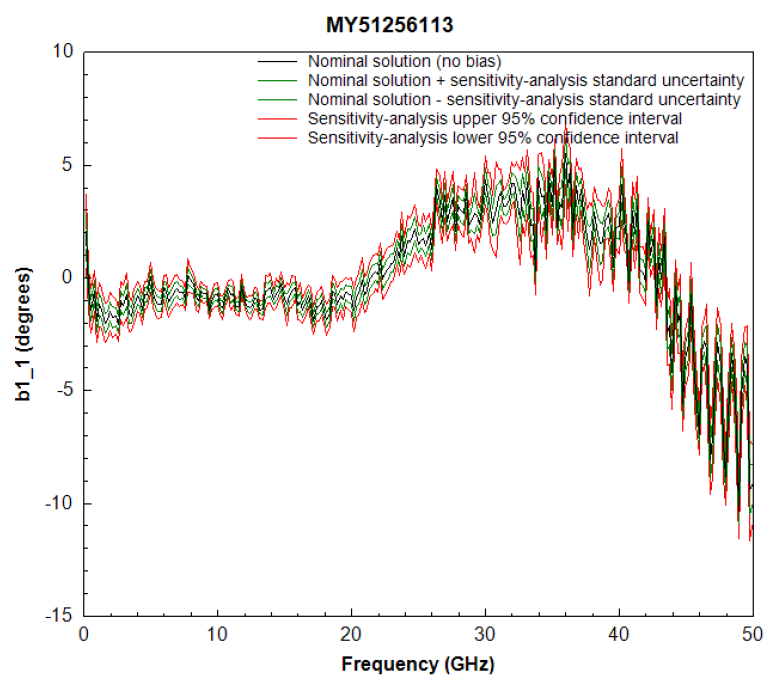
\includegraphics[width=0.62\textwidth]{combuncP.png}
		\caption{ }
	\end{subfigure}
	\caption{Results of the phase reference characterisation performed at NIST for unit MY51256113 displayed using the MUF measurement viewer software. The device was connected to port one of the NVNA performing the measurement, so the amplitude (a) and phase (b) of the b wave for the fundamental harmonic at port one (b1\_1) is shown.}
	\label{ch4_fig_combunc}
\end{figure}

\subsection{Power Meter}

Power measurement is a well-established field of electromagnetic wave metrology and is widely applied to measurements in industry as well as academia. Because of this, manufacturers have produced application notes and software to help users evaluate the uncertainty in their power meter measurements \cite{Rohde_2001, Keysight_2017}. The uncertainty evaluation presented in this project is based on the power meter measurement model used by Keysight and described in \cite{Keysight_2017}, due to the use of Keysight power meters and the fact that this model is already included in the MUF software.

The distribution of uncertainty contributions are shown in Figure \ref{ch4_fig_pmchart}. The impedance mismatch between the source to be measured and the power sensor is the dominant source of uncertainty, which is not surprising as it has a direct effect on the amount of power that reaches the sensing element.

\begin{figure}
	\centering
	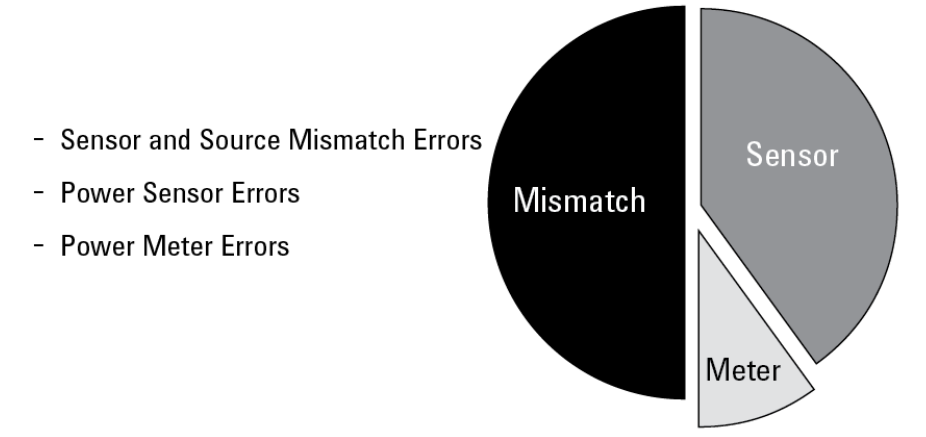
\includegraphics[width=0.7\textwidth]{pmchart.png}
	\caption{This chart shows a typical distribution of uncertainty values for its three largest causes: mismatch, sensor and meter specifications. It reveals why low SWR specifications for the power sensor and source is so crucial \cite{Keysight_2017}.}
	\label{ch4_fig_pmchart}
\end{figure}

The measurement model for the power meter can be written as

\begin{equation}
	P = \frac{M_\textrm{u}(P_\textrm{m}-t)}{K_\textrm{b}m},
\end{equation}

where $P$ is the power incident to the sensor (the measurand), $M_\textrm{u}$ is the gain due to mismatch of the power sensor, $P_\textrm{m}$ is the value given by the power meter, $t$ is the sum of offset errors including noise and zeroing errors, $K_\textrm{b}$ is the calibration factor of the power sensor, and $m$ is the sum of multiplicative errors including sensor calibration and instrumentation errors.

For an ideal measurement, $M_\textrm{u}$ and $m$ are all equal to one and $t$ is equal to zero. When the model is used with a simple evaluation of uncertainty, the worst-case values for each error can be inserted or the root-sum-of-squares (RSS) calculated to provide a range of values which the result could take. This is the propagation technique suggested in the \cite{Keysight_2017}. The MUF implementation instead sets all the input quantities to their nominal values (e.g. one or zero for the pure error terms) and instead assigns distributions to each of them. The uncertainty propagation then samples each input quantity from their distribution and obtains a sample for the measurand. A sensitivity analysis can also be performed for this model, and an example result is shown in Figure \ref{ch4_fig_pmsens}.

\begin{figure}
	\centering
	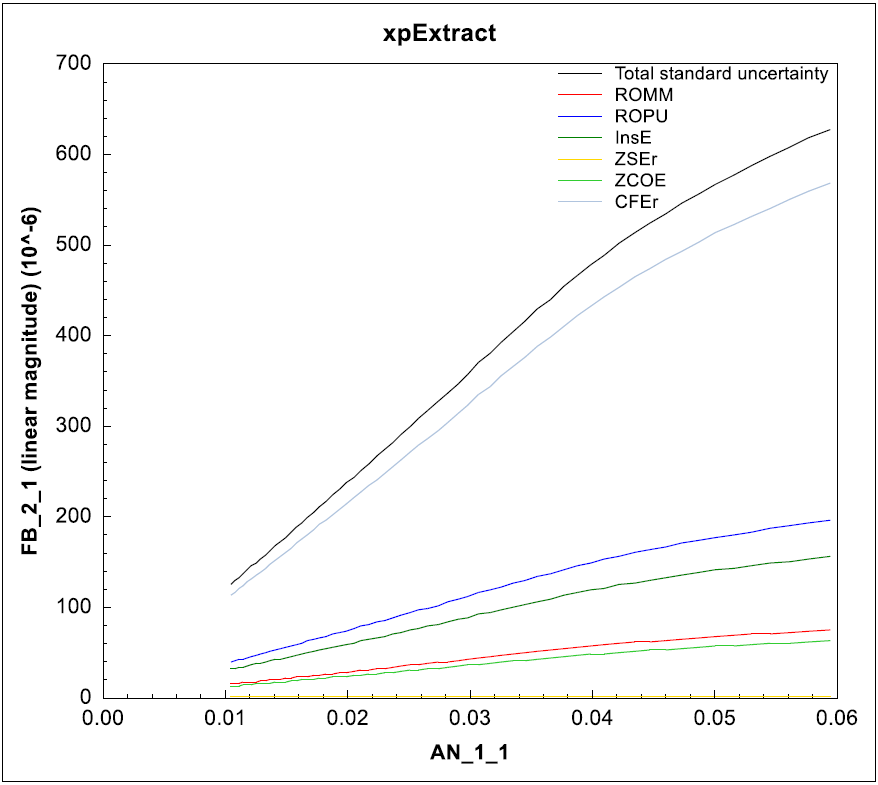
\includegraphics[width=\textwidth]{pmsens.png}
	\caption{An example sensitivity analysis showing the effect of power meter uncertainties on an X-parameter measurement. The plot shows the amplitude of the X-parameter representing the large-signal output of the amplifier into a matched load versus a swept input power. The values are in units of square-root Watts. The input quantities ROMM, ROPU and InsE all contribute to $m$, ZSEr and ZCOE contribute to $t$, and CFEr represents the error in $K_\textrm{b}$. Mismatch error is not included in the power meter model but is modelled as a cascaded adapter attached to the power sensor instead.}
	\label{ch4_fig_pmsens}
\end{figure}

\subsection{Propagation of Uncertainties}

Although there are many guides and software frameworks available for propagating uncertainty through VNA measurements, there are only two published options currently available for NVNA measurements \cite{Lin_2012, MUFWebsite}.

\subsubsection{Analytical Covariance-Based Propagation}

Lin and Zhang published a covariance-based analytical method for linear propagation of uncertainty which allows a GUM-based technique to be applied to NVNA uncertainties \cite{Lin_2012}. Partial derivates with respect to all input quantities have been derived for the NVNA measurement model, which is shown graphically in Figure \ref{ch4_fig_linmodel}. These include the use of Cauchy-Riemann derivatives in order to accommodate ratios of the complex components used to calculate magnitude and phase values for the respective parts of the absolute calibrations.

\begin{figure}
	\centering
	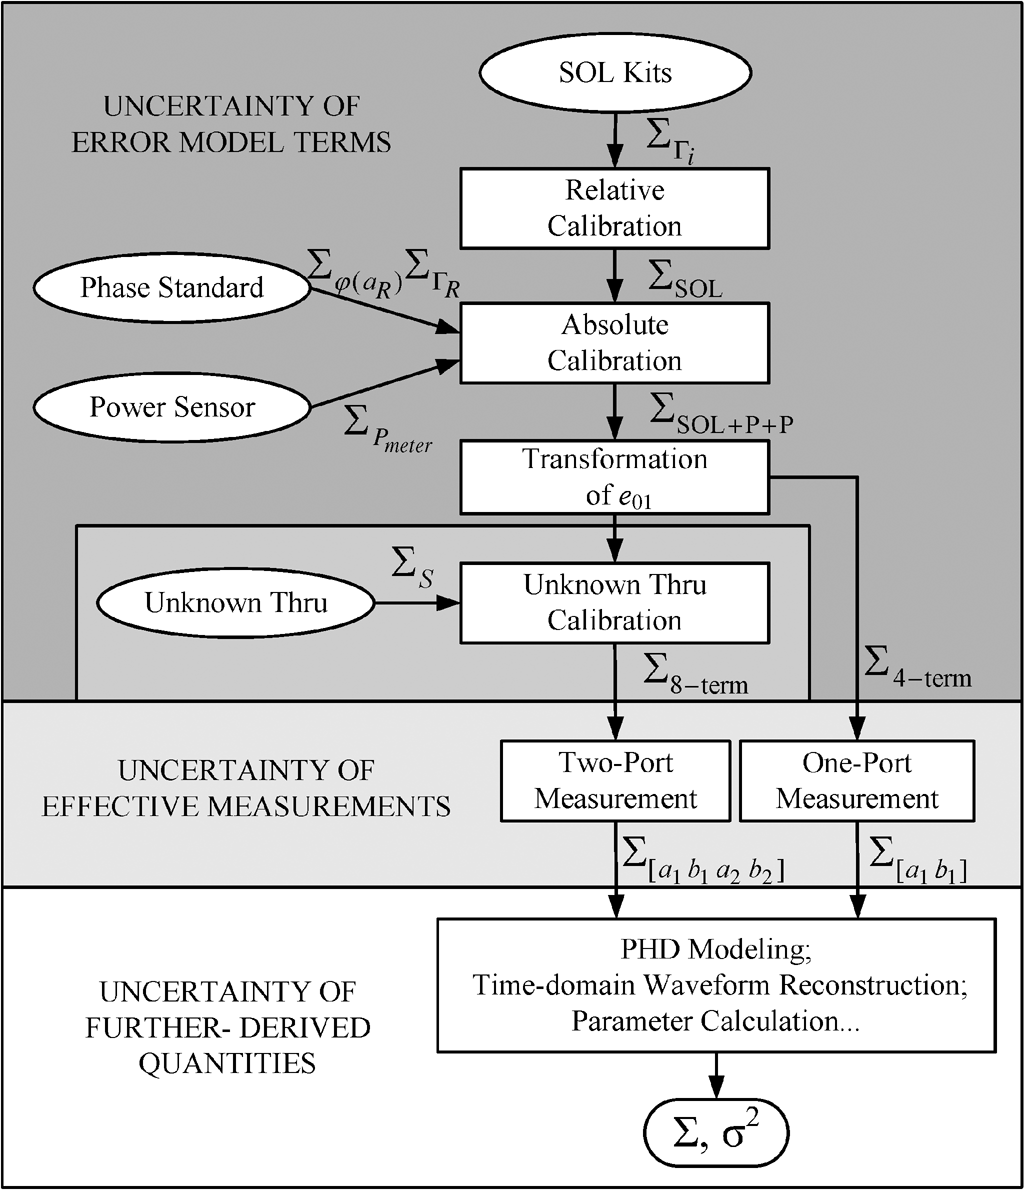
\includegraphics[width=0.8\textwidth]{linmodel.png}
	\caption{The NVNA measurement model used in \cite{Lin_2012}.}
	\label{ch4_fig_linmodel}
\end{figure}

\subsubsection{Numerical Propagation}

The MUF includes both s-parameter and wave-parameter measurement models for a VNA. The wave-parameter model was extended at NIST and used to create an NVNA measurement model which can be used to propagate uncertainty for nonlinear device measurements using the numerical methods included in the MUF - namely Monte Carlo and sequential perturbation. This was the approach chosen for the work in this project because there were already published results from this framework and it was actively supported \cite{Avolio_2015}. In addition, the MUF includes preserves information about correlations between frequencies in the form of indexed Monte Carlo samples. This is an alternative to the very large covariance matrices required to otherwise store this information at each step of the propagation (although there have been recent efforts to improve this burden using principal component compression \cite{Humphreys_2015}). This ability is significant when using the results of the measurement to produce time-domain or cross-frequency information as required by nonlinear behavioural models, where without these correlations included the combined uncertainty may be considerably perturbed.

Figure shows a screenshot of the MUF software \textbf{VNA Uncertainty Calculator} with the LSNA tab open. This part of the software allows a user to enter models for the power meter and adapters, and measurements for the power and phase calibrations. The phase reference does not use a model, but instead a characterisation file including covariances as described earlier in this section.

\begin{figure}
	\centering
	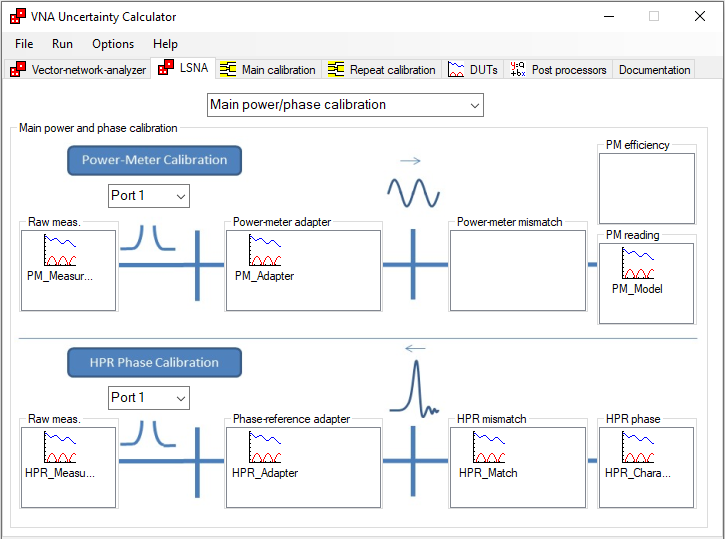
\includegraphics[width=\textwidth]{muflsna.png}
	\caption{The LSNA calibration tab of the MUF \textbf{VNA Uncertainty Calculator} application. Each file icon represents a ``.meas'' file, which contains an index of Monte Carlo samples generated from a statistical analysis of repeated measurements for each quantity. It is by this method that the MUF propagates distribution information and preserves covariance information. The power meter mismatch and efficiency input boxes are empty as they are included in the model which generated the processed power meter reading file (``PM\_Model'').}
	\label{ch4_fig_muflsna}
\end{figure}

\section{Conclusion}

This chapter has studied the application of uncertainty evaluation to measurements performed on both VNA and NVNA instruments. After a brief introduction to typical sources of uncertainty encountered in these measurements, two versions of VNA measurement models were explained. The residual error model provides a less computationally-intensive propagation of uncertainty, which was noticeably beneficial in the years when it was developed, but this concern is now less relevant. It was shown that the residual error model can also suffer from problems during the ripple measurement method used to characterise some of the input quantities, and is also not reliable when used in submillimetre-wave rectangular metallic waveguide. In contrast, the rigorous VNA measurement model provides more accurate values for combined uncertainties, especially as it correctly preserves correlations through the propagation. This can be achieved either via linear propagation methods as defined in the GUM document, or via Monte Carlo techniques as defined in the GUM supplement, both of which were explained in Chapter 3.

The extension of VNA uncertainty to NVNA measurements was also discussed, where there is a requirement to add the absolute power and phase calibrations to the VNA measurement model. Due to NVNA uncertainty evaluation being relatively young in the field of microwave metrology, there are only two available frameworks to provide such evaluations. The single software solution, the MUF, provides multiple propagation methods and includes a sensitivity analysis feature. It can propagate cross-frequency correlations which are important for use in nonlinear behavioural models. For these reasons, the MUF was selected for use in this project as the framework to use to propagate measurement uncertainty into nonlinear behavioural models.


\addcontentsline{toc}{section}{Bibliography}
\printbibliography[title=References]
\end{refsection}
\end{document}
